\documentclass{article}

\usepackage{graphicx}

\begin{document}

\title{finite mixture models}

\author{Quan Zhao}

\maketitle

% \begin{abstract}
% \textbf{If you need an abstract, then it goes here. While you are reading this document, please also criticise it for the writing style, grammar, consistency, suitability, etc. }
% \end{abstract}

% 1. Search for relevant literature - 0:30
% 2. Evaluate and select sources -  0:58
% 3. Identify themes, debates, and gaps - 1:26
% 4. Outline your literature review's structure - 1:56
% 5. Write it - 2:34

\section{Introduction}
% introduction of the research topic
% (1/2 to 1 page).

Finite mixture models are statistical models that are used to represent a population as a mixture of several subpopulations or components. These models assume that the observed data are generated from a combination of different probability distributions, each representing a distinct subpopulation within the overall population. The term "finite" in finite mixture models refers to the specific number of components or subpopulations in the mixture.

Figure~\ref{fig:trend} shows the finite mixture modelling has strong trend in publications.

\begin{figure}[h!] % 'h!' places the figure here, in the text
    \centering % Centers the figure
    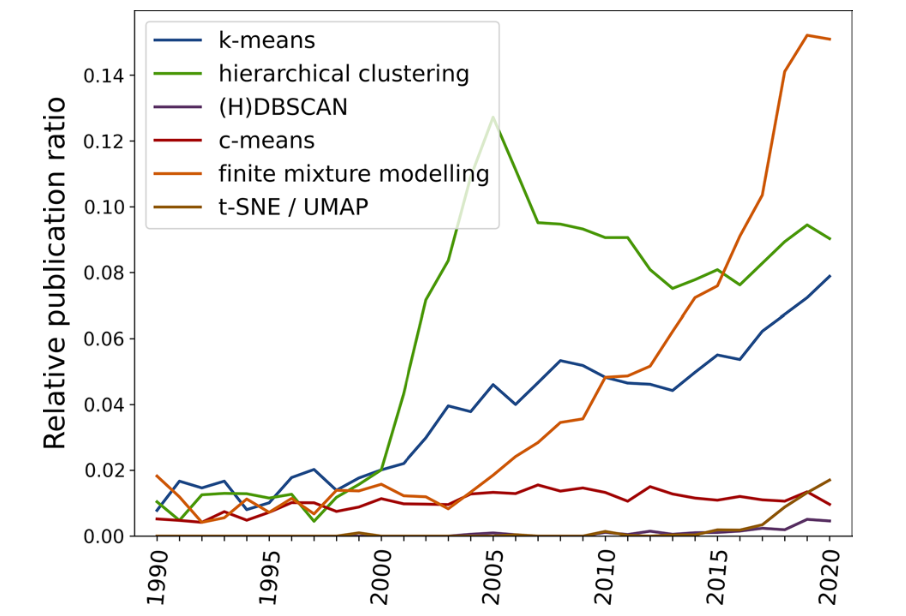
\includegraphics[width=0.6\textwidth]{images/trend.png} % Include the image with 50% of the text width
    \caption{The increase in publications indexed by PubMed that mention a keyword specific to cluster analyses relative to the number of publications 
    that mention a traditional statistical test. 
    Particularly sharp increases can be seen for finite mixture modelling.
    From~\cite{dalmaijer2022statistical}.} % Caption for the image
    \label{fig:trend} % Label for referencing the figure in the text
  \end{figure}


\section{literature review}
% The section on analysis is split into two sub-sections. 
% (about 2-3 pages)

In 2000~\cite{mclachlan2000finite} proposesed the mixture model in terms of $Y_j$ and $Z_j$ is most useful 
in that it allws the the maximum likelihood estimate (MLE) of the Mixture distribution to be computed via 
a straightforward application of the EM algorithms.
It is also useful in implementing the MCMC methods in the fitting of mixture models in a Bayesian framework.
(here, $Y_j$ is feature vector and $Z_j$ is components label vector.)

In 2016~\cite{matechou2016biclustering} proposes finite mixture models that can simultaneously cluster the rows and columns of two-mode ordinal categorical response data. The models utilize the popular proportional odds parameterization and provide insights into major patterns present in the data. Model-fitting is performed using the EM algorithm, resulting in a fuzzy allocation of rows and columns to corresponding clusters. The clustering ability of the models is evaluated through simulation studies and demonstrated using two real data sets. The paper addresses the challenge of modeling heterogeneity in two-mode ordinal data by developing finite mixture models that offer a comprehensive and interpretable approach to clustering both rows and columns, ultimately providing insights into the major patterns present in the data.

In 2016~\cite{fernandez2016mixture} introduces a new methodology for clustering rows and columns in a matrix of ordinal data. It utilizes likelihood-based methods through finite mixtures with the stereotype model. The paper demonstrates the reliability of this approach through a simulation study and further illustrates its application with two examples. Additionally, it reviews and compares several model choice measures, providing a robust framework for analyzing ordinal data matrices using fuzzy clustering techniques.

In 2019~\cite{fernandez2019finite} improved their work. It extends the finite mixture models to a broader range of data types, including binary, count, and ordinal data, under a unified statistical framework. It also introduces maximum likelihood estimation parameters and the option of using likelihood information criteria for model comparison. and it presentation of a Bayesian approach, where parameters and the number of clusters are estimated simultaneously. 

\section{Conclusions}

\bibliographystyle{plain}
\bibliography{bibliography} % Replace 'yourbibfile' with the name of your .bib file


\end{document}

